\documentclass[acmsmall,review,anonymous]{acmart}

\AtBeginDocument{%
  \providecommand\BibTeX{{%
    \normalfont B\kern-0.5em{\scshape i\kern-0.25em b}\kern-0.8em\TeX}}}

\setcopyright{acmcopyright}
\copyrightyear{2026}
\acmYear{2026}
\acmDOI{XXXXXXX.XXXXXXX}

\acmJournal{TALLIP}
\acmVolume{1}
\acmNumber{1}
\acmArticle{1}
\acmMonth{10}

\usepackage{graphicx}
\usepackage{booktabs}
\usepackage{tikz}
\usetikzlibrary{shapes.geometric, arrows, positioning, fit, backgrounds}

% Float placement parameters to prevent figures from drifting to the end
\renewcommand{\topfraction}{0.9}
\renewcommand{\bottomfraction}{0.8}
\renewcommand{\textfraction}{0.05}
\renewcommand{\floatpagefraction}{0.8}
\renewcommand{\dbltopfraction}{0.9}
\renewcommand{\dblfloatpagefraction}{0.8}
\setcounter{topnumber}{4}
\setcounter{dbltopnumber}{4}

\begin{document}

\title{Dhivehi-Bench: A Comprehensive Benchmark for Evaluating Large Language Models on the Maldivian Language}

\author{Anonymous Author(s)}
\affiliation{%
  \institution{Anonymous Institution}
  \country{Anonymous}
}

\begin{abstract}
Evaluating Large Language Models (LLMs) on low-resource languages requires datasets that are linguistically accurate, domain-diverse, and insulated from pre-training data contamination. We introduce Dhivehi-Bench, a 5,220-item multi-task benchmark for the Maldivian language (Thaana script) spanning Multiple Choice Questions (MCQ, $n=2,070$), Contextual Question Answering ($n=1,134$), and bidirectional Translation at both the sentence ($n=1,812$) and paragraph ($n=204$) levels. To prevent pre-training contamination in the comprehension tracks, we digitized historical manuscripts and academic monographs from offline physical archives using a Thaana Optical Character Recognition (OCR) pipeline and manually post-edited all extracted text before item creation. Three native Maldivian speakers independently validated every prompt-target pair under a 100\% consensus requirement. Evaluating three open-weights model families---Gemma 4 (31B), Llama 3.1 (70B), and Qwen 2.5 (72B)---reveals a consistent directional asymmetry. While Gemma 4 reaches 74.98\% accuracy on multiple-choice comprehension, 52.49\% Token F1 on extractive question answering, and 50.95 chrF when translating Dhivehi into English, all three models achieve $\leq 1.01$ word-level BLEU when generating Thaana script from English. An orthographic ablation evaluating Romanized Mal\'{e} Latin transliteration ($n=200$ stratified, with 10,000 paired bootstrap resamples) across all three model families shows that Latin output eliminates cross-script byte substitutions and cuts repetition loops on byte-fallback-bound Qwen 2.5 (from 78.5\% to 30.0\% local; 11.0\% to 4.0\% persistent), while shifting Gemma 4 into Latin grammatical particle loops (38.5\% local; 18.5\% persistent) and leaving word-level BLEU $\leq 0.26$ (15.75--18.51 chrF). A double-blind human error audit by two native speakers ($n=50$, Cohen's $\kappa=0.50$) confirms that Romanized generations remain dominated by morphological particle loops (40.0\%), lexical hallucination (37.0\%), and English code-switching (15.0\%), indicating that generative failure reflects both sub-syllabic tokenization and pre-training data scarcity.
\end{abstract}

\begin{CCSXML}
<ccs2012>
   <concept>
       <concept_id>10010147.10010178.10010179</concept_id>
       <concept_desc>Computing methodologies~Natural language processing</concept_desc>
       <concept_significance>500</concept_significance>
       </concept>
 </ccs2012>
\end{CCSXML}

\ccsdesc[500]{Computing methodologies~Natural language processing}

\keywords{Low-Resource Languages, Dhivehi, Large Language Models, Benchmarking, Dataset Construction}

\maketitle

\section{Introduction}

Scaling Large Language Models (LLMs) has improved zero-shot performance in natural language understanding and generation, yet these gains remain concentrated in high-resource, Latin-script languages. Even as multilingual benchmarks expand to cover regional macro-languages, smaller languages with distinct scripts remain largely unmeasured. Dhivehi, the Indo-Aryan national language of the Maldives spoken by approximately 400,000 people, exemplifies this gap. Written in the right-to-left Thaana script, Dhivehi rarely appears in multilingual pre-training corpora, leaving researchers without verified, uncontaminated evaluation data.

Two methodological problems complicate low-resource LLM evaluation: pre-training contamination and confounded failure modes. When benchmarks draw from public web crawls, high scores can reflect training-set memorization rather than zero-shot generalization. Conversely, when models fail on generative tasks, single-task benchmarks cannot distinguish whether the model lacks receptive comprehension of the language or fails specifically during target-script decoding.

We introduce \textbf{Dhivehi-Bench}, a 5,220-item multi-domain benchmark designed to separate receptive comprehension from autoregressive generation in the Thaana script. To insulate our reading comprehension tracks from web-crawl contamination, we digitized non-machine-readable physical archives using a fine-tuned Dhivehi OCR pipeline and manually post-edited the transcriptions before constructing evaluation items. Across multiple-choice reading comprehension, extractive question answering, and bidirectional translation, three native speakers verified every item to unanimous consensus. Our baseline evaluations on Gemma 4 (31B), Llama 3.1 (70B), and Qwen 2.5 (72B) show that open-weights models comprehend written Dhivehi far better than they generate it, tracing the generative failure to byte-level tokenization of the Thaana script.

\section{Linguistic Background: The Maldivian Language}
Dhivehi shares a genetic relationship with Sinhala inside the Southern Indo-Aryan branch, but centuries of maritime isolation and lexical contact with Arabic, Urdu, and Persian have shaped a distinct phonology, lexicon, and morphosyntax \cite{fritz_dhivehi_2002, gnanadesikan_dhivehi_2017}. Although subword modeling and acoustic cross-lingual transfer have improved Dhivehi speech recognition on Mozilla Common Voice \cite{ardila_common_2020, ahmed_improving_2023}, orthographic divergence and corpus scarcity continue to limit text-based language models \cite{zahir_expanding_2024}. 

Dhivehi is written in Thaana, a right-to-left (RTL) script developed in the Maldives that combines structural features of an abugida and a true alphabet, drawing its consonant shapes from Arabic numerals (\textit{hisaabu akuru}) and indigenous Maldivian numerals (\textit{gabulhi thaana}) \cite{gair_divehi_1996, gnanadesikan_dhivehi_2017}. Unlike the Latin alphabet, Thaana enforces obligatory diacritic stacking: every phonetic syllable pairs a base consonant (\textit{akuru}) with a mandatory vowel diacritic (\textit{fili}) placed directly above or below the consonant across 24 primary consonants and 11 vowel diacritics \cite{gnanadesikan_dhivehi_2017}. When a consonant carries no vowel sound, it takes a \textit{sukun} diacritic (\texttt{U+07B0}) to mark vowel absence in syllable codas or consonant gemination. The sole structural exception in standard Thaana orthography is \textit{Hus Noonu} (``bare Noonu''), where the consonant \textit{Noonu} (\texttt{U+0782}) appears without any vowel diacritic or \textit{sukun} to mark prenasalization of a following voiced stop (\textit{d}, \textit{dh}, \textit{b}, or \textit{g}, as in \textit{kandu} [sea] or \textit{handhu} [moon]); by contrast, a \textit{Noonu} carrying a \textit{sukun} marks a full nasal coda or geminate \cite{gair_divehi_1996, gnanadesikan_dhivehi_2017}. These conventions strain automated pipelines: general-purpose OCR models insert spurious diacritics over bare \textit{Hus Noonu}, while byte-fallback tokenizers split consonant-diacritic syllables into unmerged byte sequences.

Grammatically, Dhivehi is agglutinative, appending tense, plurality, definiteness, and case suffixes to root words \cite{fritz_dhivehi_2002, gnanadesikan_dhivehi_2017}. A single nominal stem inflects through sequential suffixation: the noun \textit{rah} (island, stem \textit{rash-}) becomes \textit{rahthah} (islands) and \textit{rahthakuge} (of the islands), mapping a single Dhivehi word to a multi-word English prepositional phrase. In autoregressive generation, mispredicting a single trailing diacritic changes the grammatical case or definiteness of the entire word.

\section{Related Work}

\subsection{Macro-Language vs. Micro-Language Benchmarking}
Multilingual benchmarks have expanded substantially since 2022, yet coverage remains uneven across script families. The Aya Project \cite{ustun_aya_2024} established multilingual instruction-tuning baselines across 101 languages, while SERENGETI \cite{adebara_serengeti_2023}, FLORES-200 \cite{team_no_2022}, and Belebele \cite{bandarkar_belebele_2024} created evaluation suites for translation and reading comprehension across up to 200 languages. Despite their scale, both FLORES-200 and Belebele's 122-language reading comprehension benchmark omit Dhivehi, and no public multi-task suite evaluates reading comprehension or extractive question answering in Thaana. The NLLB-200 translation model and the FLORES-200 benchmark share a single list of 202 language variants across 28 scripts, and neither includes Dhivehi or the Thaana script. The identifier \texttt{div\_Thaa} appears only in later resources that adopted NLLB's naming scheme, such as the FineWeb-2 pre-training corpus \cite{penedo_fineweb2_2025}. Within South Asia, IndicGenBench \cite{singh_indicgenbench_2024}, IndicQA \cite{singh_indic_2025}, and MILU \cite{verma_milu_2025} evaluate major mainland Indic languages such as Hindi, Bengali, and Tamil, leaving insular scripts like Thaana unrepresented. Dhivehi-Bench fills this gap with a multi-task suite tailored to Dhivehi orthography and morphology.

\subsection{Data Contamination in LLM Evaluation}
Web-scraped benchmarks risk overlap with pre-training corpora such as Common Crawl. Chen et al. \cite{chen_benchmarking_2025} and Dong et al. \cite{dong_generalization_2024} demonstrate that evaluating LLMs on contaminated test sets inflates zero-shot metrics through memorization rather than generalization. To counter pre-training leakage, Li et al. \cite{li_latesteval_2023} recommend constructing benchmarks from newly digitized or post-cutoff sources. We apply this offline sourcing strategy to Dhivehi-Bench's comprehension tracks, digitizing non-machine-readable physical archives through the Viyavi OCR pipeline \cite{hameed_bridging_2026} so that source passages do not overlap with existing web crawls.

\subsection{Tokenization Disparity in Morphologically Rich Languages}
Subword tokenizers such as Byte-Pair Encoding (BPE) \cite{sennrich_neural_2016} and SentencePiece \cite{kudo_sentencepiece_2018} allocate vocabulary merges according to training corpus frequency, penalizing non-Latin scripts \cite{ahia_all_2023, petrov_language_2023, rust_how_2021}. Although Arnett et al. \cite{arnett_evaluating_2025} find that morphological boundary alignment alone explains little performance variance across 70 languages, Pawar et al. (\textit{Broken Words, Broken Performance} \cite{pawar_broken_2025}) show that severe subword and byte fragmentation inflates sequence lengths and degrades autoregressive generation. Benchmarks for Extremely Low-Resource Languages (ELRLs), including IrokoBench \cite{adelani_irokobench_2025} across 16 African languages and FormosanBench \cite{lin_formosanbench_2025} across Indigenous Taiwanese languages, report similar drops on generative tracks when token fertility rises.

Several tokenization reforms target this fragmentation. MorphBPE \cite{asgari_morphbpe_2026} and Morpheme-Aware Subword Construction (MoVoC) \cite{teklehaymanot_movoc_2025} constrain BPE merges to respect morpheme boundaries, while SCRIPT-BPE \cite{land_bpe_2025} and MYTE \cite{limisiewicz_myte_2024} modify pretokenization and byte encoding to prevent cross-byte splitting in non-Latin scripts. At the architectural level, Byte Latent Transformer \cite{pagnoni_byte_2025} and H-Net \cite{hwang_dynamic_2025} replace fixed subword vocabularies with dynamic byte-to-patch grouping. Dhivehi-Bench tests how standard subword tokenizers behave when generating a script with zero learned multi-character merges.

\subsubsection{Implications for Transformer Self-Attention}
High token fertility directly elongates the sequence over which self-attention operates, where computational complexity scales as $O(N^2)$ with sequence length $N$. Because the Thaana Unicode block (\texttt{U+0780--U+07BF}) requires two bytes per codepoint in UTF-8, a 10-codepoint inflected Dhivehi word such as \textit{rahthakuge} (``of the islands'') expands into up to 20 byte- or character-level tokens when the tokenizer lacks Thaana merges. Spreading a single word across 20 positional embeddings forces attention heads to track multi-step byte reconstruction alongside clause-level syntax. Building on Holtzman et al.'s analysis of neural text degeneration under greedy decoding \cite{holtzman_curious_2020}, we hypothesize that this sequence inflation increases susceptibility to repetition loops: as byte sequences lengthen, small probability perturbations trap the autoregressive decoder in repetitive local minima.

\subsection{Prior Dhivehi NLP Infrastructure}
Published NLP tools for Dhivehi consist primarily of Mismaah's rule-based stemming and morphological utilities \cite{mismaah_dhivehi_nlp_2023}, Ahmed's subword-modeled Automatic Speech Recognition (ASR) pipeline on Mozilla Common Voice \cite{ardila_common_2020, ahmed_improving_2023}, and Zahir and Riyaz's corpus construction studies \cite{zahir_expanding_2024}. While Burmese-SAN \cite{aung_burmese-san_2026} and UrduBench \cite{shafique_urdubench_2026} have established human-curated LLM evaluation suites for other low-resource Asian scripts, Dhivehi has lacked a public multi-task benchmark.

\section{Dhivehi-Bench Dataset Construction}
\label{sec:dataset}

We designed the Dhivehi-Bench curation pipeline to pair offline archival reading comprehension tracks with a verified bilingual translation track (Figure \ref{fig:pipeline}).

\begin{figure*}[t]
\centering
\resizebox{0.95\textwidth}{!}{
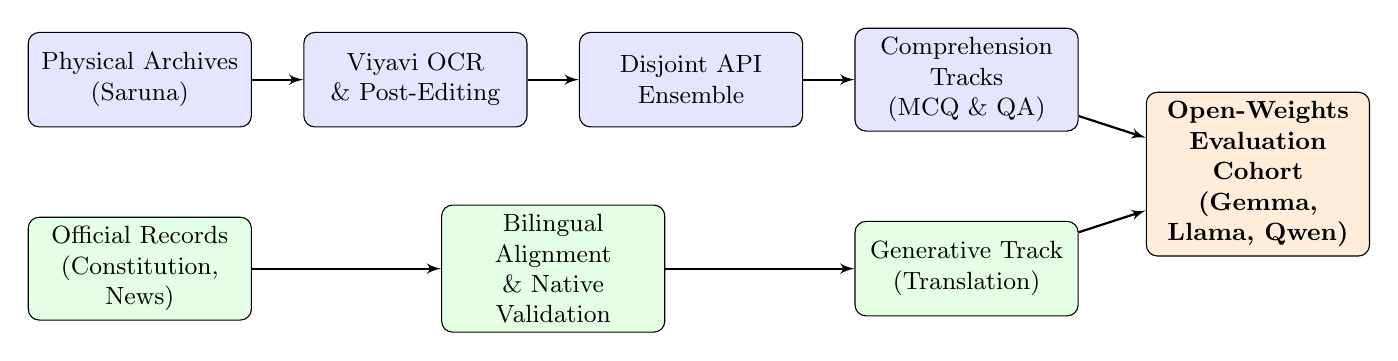
\begin{tikzpicture}[
    block/.style={rectangle, draw, fill=blue!10, text width=2.6cm, text centered, rounded corners, minimum height=1.2cm, font=\small},
    block_mt/.style={rectangle, draw, fill=green!10, text width=2.6cm, text centered, rounded corners, minimum height=1.2cm, font=\small},
    eval/.style={rectangle, draw, fill=orange!15, text width=2.6cm, text centered, rounded corners, minimum height=1.2cm, font=\bfseries\small},
    line/.style={draw, -latex', thick}
]
% Stream 1: Offline Contamination-Controlled Track (MCQ & QA)
\node [block] (archives) at (0, 1.2) {Physical Archives\\(Saruna)};
\node [block] (ocr) at (3.5, 1.2) {Viyavi OCR\\\& Post-Editing};
\node [block] (ensemble) at (7.0, 1.2) {Disjoint API\\Ensemble};
\node [block] (comp_tracks) at (10.5, 1.2) {Comprehension Tracks\\(MCQ \& QA)};

% Stream 2: Bilingual Translation Track (MT)
\node [block_mt] (mt_source) at (0, -1.2) {Official Records\\(Constitution, News)};
\node [block_mt] (mt_align) at (5.25, -1.2) {Bilingual Alignment\\\& Native Validation};
\node [block_mt] (trans_track) at (10.5, -1.2) {Generative Track\\(Translation)};

% Evaluation Cohort Node
\node [eval] (eval) at (14.2, 0) {Open-Weights\\Evaluation Cohort\\(Gemma, Llama, Qwen)};

% Paths for Stream 1
\path [line] (archives) -- (ocr);
\path [line] (ocr) -- (ensemble);
\path [line] (ensemble) -- (comp_tracks);
\path [line] (comp_tracks) -- (eval);

% Paths for Stream 2
\path [line] (mt_source) -- (mt_align);
\path [line] (mt_align) -- (trans_track);
\path [line] (trans_track) -- (eval);

\end{tikzpicture}
}
\caption{The Dual-Stream Curation Pipeline of Dhivehi-Bench. To mitigate pre-training contamination in reading comprehension, source texts for MCQ and Contextual QA are digitized from offline physical archives via custom OCR and post-edited before candidate generation via an API ensemble. The Translation track is curated from official bilingual records and verified by native speakers to examine script-conditioned generation.}
\label{fig:pipeline}
\end{figure*}

\subsection{Anti-Contamination via Custom OCR Digitization}
We drew the source passages for the reading comprehension and question-answering tracks from the Maldives National University's Digital Repository (\textit{Saruna}), downloading scanned, non-machine-readable PDFs and manuscripts from the ``Dhivehi Language Studies'' and eight related archival collections containing historical essays, monographs, and legal treatises.

We digitized these scans using the open-source Viyavi Multi-Scale OCR series \cite{hameed_bridging_2026}, a Vision-Language Model suite fine-tuned on the Qwen-2.5 architecture for the Thaana script. Because Thaana writes right-to-left and stacks vowel diacritics (\textit{fili}) above and below base consonants (\textit{akuru}), general-purpose OCR engines routinely drop diacritics or missegment characters. On held-out historical manuscripts, the 3B Viyavi model achieved an 8.0\% Character Error Rate (CER). To eliminate residual recognition errors before question drafting, native speakers manually post-edited all OCR transcriptions. A secondary audit on a held-out sample of 300 post-edited lines measured a residual CER of 1.4\% and a Word Error Rate (WER) of 3.2\%, reflecting minor diacritic conventions in manual Thaana transcription while confirming that initial OCR errors were resolved prior to item creation.

\subsection{Task Taxonomy and Manual Curation}
\label{sec:taxonomy}
Dhivehi-Bench comprises three evaluation tracks:
\begin{itemize}
    \item \textbf{Multiple Choice Questions (MCQ, 2,070 items):} We constructed the reading comprehension track through a hybrid human-AI curation workflow. First, the \textit{Dhivehi-English Alignment Engine} drafted candidate questions, target answers, and three distractors from the post-edited archival passages. To avoid single-model stylistic bias, we distributed candidate drafting across three commercial APIs: Gemini 3.8 Flash, GPT-4o, and Claude 3.5 Sonnet. Although this drafting ensemble (Gemini, GPT-4o, Claude) does not include Llama 3.1 or Qwen 2.5, Gemma 4 shares architectural, tokenizer, and distillation lineage with Google's Gemini family. Direct item-level memorization is nonetheless prevented because all source passages originate from offline archival scans, and native human annotators screened every candidate item, discarding 23.0\% of the initial MCQ pool and editing surviving options where needed.

We managed candidate review in a custom Curation Interface using a two-stage, three-evaluator filtering workflow. A natural methodological question arises: \textit{how could commercial LLMs draft usable Thaana candidate questions when the evaluated open-weights models fail at English-to-Dhivehi translation?} Two task-level factors account for this difference. First, whereas zero-shot $\text{EN}\rightarrow\text{DV}$ translation provides only Latin-script English in the prompt and requires the decoder to generate Thaana from scratch, the MCQ and QA drafting prompts included the human post-edited Dhivehi (Thaana) archival paragraph directly in the context window. Drafting short questions, answer spans, and options from an in-context Dhivehi passage functions primarily as \textit{in-context span-copying and lexical recombination}, allowing attention heads to copy character sequences directly from the input passage (aided by proprietary tokenizers and server-side repetition controls in the commercial APIs). Second, raw candidate generations still contained frequent orthographic or factual errors. From an initial pool of 2,688 LLM-drafted MCQ candidates, two native Maldivian evaluators screened each item against its source paragraph and discarded 618 malformed, repetitive, or ungrounded questions (a 23.0\% rejection rate), editing surviving distractors where needed to ensure morphological plausibility and resolve diacritic errors. A third independent native evaluator reviewed and confirmed the remaining 2,070 items to reach unanimous consensus.
    \item \textbf{Contextual Question Answering (1,134 items):} Modeled on extractive reading comprehension benchmarks such as SQuAD \cite{rajpurkar_squad_2016} and TyDi QA \cite{clark_tydi_2020}, this track pairs digitized \textit{Saruna} paragraphs with questions whose answers appear as contiguous spans in the passage. The 1,134 validated items span nine archival collections summing to 100.0\%: Dhivehi Language Studies (49.6\%, $n=563$, avg context 154.5 words), Literature \& Poetry (24.6\%, $n=279$, avg context 79.5 words), Religion \& Islam (10.2\%, $n=116$, avg context 75.7 words), Shariah \& Law (4.1\%, $n=46$, avg context 66.7 words), Political Science (3.2\%, $n=36$, avg context 168.7 words), Maldivian History (3.0\%, $n=34$, avg context 73.7 words), General Knowledge (2.1\%, $n=24$, avg context 79.6 words), Science \& Geography (1.9\%, $n=22$, avg context 77.3 words), and Art \& Culture (1.2\%, $n=14$, avg context 61.6 words). Starting from 2,162 candidate QA pairs, two native evaluators removed 388 defective or context-independent pairs (retaining 1,774 items); enforcing a density cap of 3 items per source paragraph and final adjudication by the third native evaluator yielded 1,134 items (a 47.5\% total rejection rate, with 1,028 candidates discarded).
    \item \textbf{Translation (2,016 pairs; Sentence and Paragraph Levels):} To test generation across two discourse lengths, we curated 2,016 parallel English-Dhivehi pairs divided into 1,812 single-sentence items (averaging 20.2 English source words) and 204 multi-sentence paragraph excerpts (averaging 27.5 English source words, ranging up to 110 words). We collected these parallel texts from official Maldivian Presidency press releases, the Constitution of the Maldives, and published non-fiction and literary translations, aligning segments with the \textit{Dhivehi-English Alignment Engine} before full manual verification by native speakers. Unlike the offline archival comprehension tracks, these public-domain texts may appear in web-scale pre-training corpora. That exposure strengthens our diagnostic finding: even when models have seen the English source texts during pre-training, their output collapses when translating into Thaana, isolating target-script decoding rather than source-text comprehension as the point of failure.
\end{itemize}

\subsection{Corpus Statistics}
\label{sec:corpus_stats}
Table \ref{tab:stats} reports word and item counts across the three tracks. Across all source contexts, prompts, and target references, Dhivehi-Bench totals 280,091 words (239,431 source words and 40,660 target words, or over 273,000 non-overlapping words when excluding extractive QA answer spans that also appear inside source contexts).

\begin{table*}[t]
\centering
\caption{Dhivehi-Bench Corpus Statistics.}
\label{tab:stats}
\begin{tabular}{lccc}
\toprule
\textbf{Evaluation Track} & \textbf{Total Prompts} & \textbf{Total Source Words} & \textbf{Total Target Words} \\
\midrule
Multiple Choice (MCQ) & 2,070 & 54,626 & N/A (Discrete Choice) \\
Contextual QA (SQuAD-style) & 1,134 & 142,662 (Context + Q) & 6,258 (Answer Spans) \\
Translation (1,812 sent. / 204 para.) & 2,016 & 42,143 (English) & 34,402 (Dhivehi) \\
\bottomrule
\end{tabular}
\end{table*}

\subsection{Quality Assurance and Annotation Protocol}
Because Dhivehi lacks automated grammatical parsers, three native Maldivian speakers verified every item across the MCQ, Contextual QA, and Translation tracks. Two primary evaluators conducted initial context-grounding checks, distractor rewriting, and candidate filtering, and a third independent evaluator performed final adjudication. All three annotators completed formal secondary education in the Maldives, where Dhivehi grammar, literature, and orthography are compulsory curriculum subjects. Because shifting a single vowel diacritic changes lexical meaning or grammatical case, we required 100\% agreement across all three annotators to retain an item. All evaluators participated with informed consent and were compensated fairly according to local Maldivian professional and academic rates.

\section{Evaluation Methodology and Baselines}
We evaluated three open-weights foundation models spanning distinct model families and parameter scales: Gemma 4 (31B) \cite{team_gemma_2026}, Llama 3.1 (70B) \cite{grattafiori_llama_2024}, and Qwen 2.5 (72B) \cite{qwen_qwen25_2025}. Evaluating open-weights checkpoints guarantees deterministic reproducibility and provides direct access to token log-likelihoods for multiple-choice scoring. We exclude dedicated encoder-decoder translation models from the main multi-task table because they cannot perform zero-shot MCQ or extractive QA. NLLB-200 \cite{team_no_2022} cannot serve even as a translation reference. Its 600M, 1.3B, and 3.3B checkpoints share a 256,204-token SentencePiece vocabulary with no \texttt{div\_Thaa} language tag and no Thaana consonants. Because the tokenizer has no byte fallback, every Thaana consonant in the input maps to \texttt{<unk>} (token ID 3; Table \ref{tab:tokenizer_vocab}). We therefore use MADLAD-400 (7B) \cite{kudugunta_madlad-400_2023}, which includes Dhivehi among its training languages, as the translation reference. On the EN$\rightarrow$DV track it scored 6.8 BLEU and 38.2 chrF. MADLAD-400 does not produce the repetition loops seen in the causal LLMs, but its training data include public web crawls that overlap with Maldivian constitutional and government texts.

\subsection{EleutherAI Evaluation Harness and Log-Likelihood}
We ran all evaluations through EleutherAI's \textit{lm-evaluation-harness} \cite{gao_framework_2023} under a fixed random seed ($\text{seed}=42$), using the standardized task prompt templates documented in Appendix A.

For the MCQ track, we scored models via length-normalized conditional log-likelihood (\texttt{acc\_norm} in the EleutherAI harness), dividing the log-probability of each candidate option by its byte-token length so that subword fragmentation does not penalize longer Dhivehi options. In the raw curation export, target answer keys skewed toward early slots (Option A: 46.81\%, Option B: 37.58\%, Option C: 14.78\%, Option D: 0.82\%) because the curation UI initialized candidate answers in slot A before annotator reassignment. To remove positional bias, the benchmark release permutes option positions using $\text{seed}=42$ to enforce an exact 25.0\% distribution across Options A, B, C, and D.

\subsection{The Tokenization Tax: Byte-Fallback and Fertility Metrics}
\label{sec:tokenization_tax}

\begin{figure*}[!t]
\centering
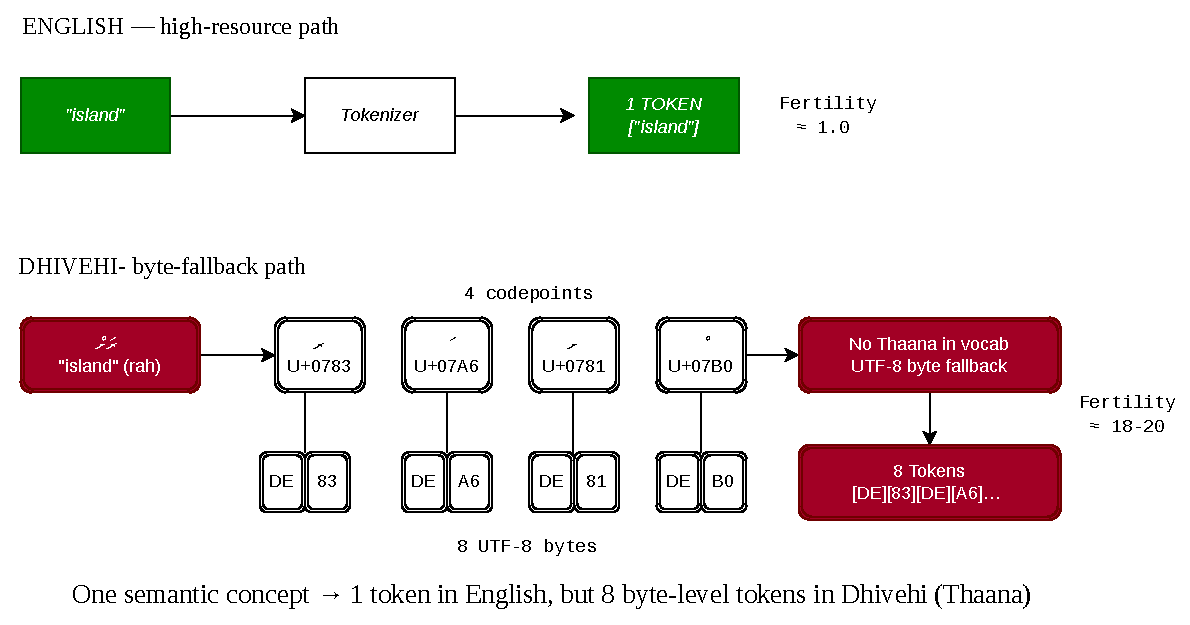
\includegraphics[width=0.9\linewidth]{fig_tokenization.pdf}
\caption{The Tokenization Tax. While an English word encodes to a single token, its Dhivehi counterpart is segmented into 8 byte-level tokens due to the lack of learned Thaana subword merges, obscuring morphological boundaries.}
\label{fig:tokenization}
\end{figure*}

To test how tokenizer vocabularies represent Dhivehi, we inspected the vocabulary files and measured token fertility across all three evaluated models over the Thaana Unicode block (\texttt{U+0780}--\texttt{U+07BF}).

We define our counting criterion explicitly: \textit{a vocabulary entry counts as a Thaana token if and only if its decoded UTF-8 representation contains at least one codepoint in \texttt{U+0780}--\texttt{U+07BF}, and a multi-character merge is any single token whose decoded bytes represent two or more Thaana codepoints.} Our companion repository includes the verification script (\texttt{scripts/verify\_tokenizers.py}) with pinned Hugging Face revisions (Gemma 4/2: \texttt{33c1930284}, Llama 3.1: \texttt{d04e592bb4}, Qwen 2.5: \texttt{d149729398}).

None of the three tokenizers contains a single learned multi-character merge for Dhivehi (Table \ref{tab:tokenizer_vocab}). Gemma 4 uses a base SentencePiece \cite{kudo_sentencepiece_2018} unigram vocabulary of 256,000 tokens \cite{team_gemma_2026}, with its output embedding and Multi-Token Prediction (MTP) projection layer padded to $d \times 262,144$ ($2^{18}$) for hardware alignment. Although Gemma 4 includes 42 isolated single-codepoint Thaana characters and Qwen 2.5 \cite{qwen_qwen25_2025} includes 8 isolated single consonants, both models contain 0 multi-character Thaana merges. Llama 3.1 (128,256 tokens) \cite{grattafiori_llama_2024} contains 0 Thaana tokens of any kind.

Because written Dhivehi requires diacritic stacking---attaching a vowel diacritic (\textit{fili}) above or below every base consonant---an isolated consonant cannot form a phonetic syllable. With zero consonant+\textit{fili} merges, continuous Dhivehi text fragments below the syllable level into unmerged single codepoints and raw UTF-8 fallback bytes. Llama 3.1 splits 100\% of Thaana characters into two UTF-8 byte tokens; Qwen 2.5 falls back to two UTF-8 bytes for all vowel diacritics and 16 of the 24 primary consonants; and Gemma 4 splits inflected Dhivehi words into sequences of 20 or more unmerged character and byte tokens.

\begin{table}[t]
\centering
\small
\setlength{\tabcolsep}{3.5pt}
\caption{Tokenizer Architecture and Empirical Thaana Coverage Across Evaluated Models. A token is classified as Thaana if its decoded UTF-8 byte representation contains codepoints in \texttt{U+0780}--\texttt{U+07BF}. Across open-weights models, multi-character Thaana merges are zero, resulting in sub-syllabic and byte-level fragmentation on continuous text, while NLLB-200 collapses to \texttt{<unk>} due to missing Thaana vocabulary and lack of byte fallback.}
\label{tab:tokenizer_vocab}
\begin{tabular}{llcccc}
\toprule
\textbf{Model} & \textbf{Tokenizer Family} & \textbf{Base Vocab} & \textbf{Effective Vocab} & \textbf{Thaana Tokens} & \textbf{Multi-Char Merges} \\
\midrule
Gemma 4 (31B) & SentencePiece & 256,000 & 262,144\textsuperscript{*} & 42 & 0 \\
Llama 3.1 (70B) & Tiktoken BPE & 128,000 & 128,256 & 0 & 0 \\
Qwen 2.5 (72B) & Tiktoken BPE & 151,643 & 152,064 & 8\textsuperscript{\dag} & 0 \\
NLLB-200 (600M--3.3B) & SentencePiece & 256,204 & 256,204 & 1\textsuperscript{\ddag} & 0 \\
\bottomrule
\end{tabular}
\begin{flushleft}
\footnotesize
\textsuperscript{*} The base SentencePiece unigram vocabulary is 256,000; the architectural embedding and projection layers are dimensioned to $d \times 262,144$ ($2^{18}$, $\approx 262\text{k}$) in the Gemma Technical Report \cite{team_gemma_2026}.\\
\textsuperscript{\dag} Qwen 2.5 includes 8 isolated single-consonant characters without vowel diacritics (\textit{fili}); because written Dhivehi requires consonant-vowel combinations, continuous text relies on byte fallback.\\
\textsuperscript{\ddag} NLLB-200 contains zero Thaana consonants (only 1 isolated vowel diacritic \texttt{U+07AC}) and omits \texttt{div\_Thaa}; lacking byte-fallback, all Dhivehi text collapses to \texttt{<unk>}.
\end{flushleft}
\end{table} 

Measuring token fertility (tokens per whitespace-delimited word) across all 2,016 parallel translation pairs quantifies this expansion. On English text, Gemma 4 averages 1.28 tokens/word, whereas on the parallel Dhivehi text it averages 21.12 tokens/word---a 16.50x fertility ratio. Llama 3.1 reaches a 15.04x ratio (1.33 English vs. 20.00 Dhivehi tokens/word), and Qwen 2.5 reaches a 14.59x ratio (1.22 English vs. 17.80 Dhivehi tokens/word). Generating a 100-word Dhivehi passage therefore requires predicting more than 2,000 sequential tokens (Figure \ref{fig:tokenization}).

\subsection{Unconstrained Evaluation Framework and Decoding Strategy}
Because 14.6x--16.5x token fertility causes standard generation limits to truncate Dhivehi outputs mid-sentence, we set unconstrained generation ceilings across the Thaana benchmark tracks: $\text{max\_tokens} = 8,192$ for Gemma 4 $\text{EN}\rightarrow\text{DV}$ translation and MCQ, and $\text{max\_tokens} = 1,024\text{--}2,048$ for Llama 3.1 and Qwen 2.5 translation, Contextual QA, and $\text{DV}\rightarrow\text{EN}$ runs (whereas the single-sentence Romanized Mal\'{e} Latin ablation in \S\ref{sec:ablation-romanized} uses $\text{max\_tokens} = 256$, matching the word-level capacity of $\ge 1,024$ Thaana tokens under 1.5--2.0 Latin tokens/word). Across all generative evaluations, we used deterministic greedy decoding (\(\text{temperature} = 0.0\)) without custom stop-sequences so that repetition loops reflect deterministic decoder behavior rather than sampling noise.

\subsection{Agglutinative Text Normalization and Span Granularity}
Following standard extractive QA evaluation protocols \cite{rajpurkar_squad_2016, clark_tydi_2020}, our Contextual QA scoring pipeline strips ASCII punctuation while preserving all Thaana vowel diacritics (\textit{fili}). Across evaluated models, Exact Match (EM, 3.00\%--14.55\%) trails Token F1 (22.58\%--52.49\%) by up to 38 percentage points, and even strong models plateau near 52.5\% Token F1. Inspecting the predictions and reference spans identifies three linguistic and dataset factors behind this ceiling: (i) \textit{span-boundary granularity}, where single references in the dataset alternate between minimal noun-phrase entities (e.g., \textit{roanunneve} [``from coir rope'']) and full framing clauses that repeat the question stem (\textit{kaabafain mivaa alhai ulhunee roanunneve} [``ancestors wove this rope from coir'']), penalizing concise entity extractions against clause-level references and vice versa; (ii) \textit{agglutinative suffixation and copula attachment}, where stand-alone answers attach the sentence-final copula (\textit{-eve}) or drop mid-sentence case suffixes (\textit{rah} vs. \textit{rashaku}) present in the source passage; and (iii) \textit{orthographic compound spacing}, where writers vary in joining or separating prefixes and postpositions (e.g., \textit{bey-ihuthiyaarugaeve} written as one token vs. two whitespace-delimited tokens).

\subsection{Human Baseline Validation}
\label{sec:human_baseline}
To establish an empirical human reference and test how single-reference span granularity affects native speakers, a native Maldivian speaker with formal secondary education in Dhivehi completed a stratified 200-item subset (100 MCQ, 100 Contextual QA) without access to reference keys or model outputs. On the MCQ track, the human evaluator achieved 90.00\% accuracy (90/100), establishing a 15.0-point ceiling above the strongest open-weights model (Gemma 4 at 74.98\%). On Contextual QA, however, scoring the human evaluator's responses under strict whitespace SQuAD matching yielded 52.64\% Token F1 and 18.00\% Exact Match (20.00\% after stripping Thaana commas)---nearly identical to Gemma 4 (52.49\% Token F1, 14.55\% EM).

Auditing the 100 human responses against the references suggests that most of the gap between the 90.00\% MCQ score and the 52.64\% QA F1 comes from span boundaries and orthography rather than misreading. Twenty responses match the reference exactly after normalization. Thirty-three are sub-spans or super-spans of it, for example the bare entity where the reference repeats the question stem. Thirty-five share at least one token with it, typically the same root with a different suffix or spacing. Only twelve share no token with the reference or were left blank. The same audit over all 1,134 items gives Gemma 4 (31B) a similar profile (14.9\% exact, 33.9\% sub- or super-span, 39.1\% partial overlap), compared with 26.7\% total overlap for Llama 3.1 (70B) and 19.6\% for Qwen 2.5 (72B). Partial overlap is a loose criterion and does not by itself establish correctness. Still, the similarity between the human and Gemma 4 profiles indicates that strict single-reference F1 understates both.

\subsection{Metrics}
On the MCQ track ($n=2,070$), length-normalized accuracy has a 95\% confidence interval of $\pm 2.2\%$. On Contextual QA ($n=1,134$), we report Exact Match (EM) and Token-level F1.

On the Translation track ($n=2,016$), we pair word-tokenized sacreBLEU \cite{post_call_2018} (\texttt{nrefs:1|\allowbreak case:mixed|\allowbreak eff:no|\allowbreak tok:13a|\allowbreak smooth:exp|\allowbreak version:2.3.1}) with character-tokenized BLEU (\texttt{tok:char}, reported as char-BLEU in \S\ref{sec:domain_granularity}) and chrF \cite{popovic_chrf_2015}. Because agglutinative suffixation penalizes whole-word matching under \texttt{tok:13a}, chrF serves as our primary translation metric. We also report \textit{Loop Rate}, defined as the percentage of outputs that repeat an identical 4-gram $\geq50$ times; across the 2,016-item $\text{EN}\rightarrow\text{DV}$ track, Gemma 4 records a 3.6\% persistent Loop Rate (ranging from 3.3\% on general prose to 5.7\% on constitutional law; \S\ref{sec:domain_granularity}), while our qualitative error analysis (\S\ref{sec:qualitative_errors}) reveals that repetitive loops characterize 28.0\% of all generation failures alongside cross-script substitutions and broken morphology. We omit neural metrics such as COMET \cite{rei_comet_2020} because their underlying encoders (e.g., XLM-RoBERTa) lack Thaana vocabulary coverage.

\section{Results and Discussion}

\subsection{Benchmark Results}
Table \ref{tab:results} reports baseline performance across all four task directions: MCQ, Contextual QA, $\text{EN}\rightarrow\text{DV}$ translation, and $\text{DV}\rightarrow\text{EN}$ translation.

\begin{table*}[t]
\centering
\small
\setlength{\tabcolsep}{4.5pt}
\caption{Dhivehi-Bench Baseline Evaluation Results for Open-Weights Models. Translation scores reflect EN$\rightarrow$DV (generating Thaana) and DV$\rightarrow$EN (generating English) to examine Receptive Bilingualism. All MCQ evaluations are computed via length-normalized log-likelihood. On Contextual QA, strict whitespace Token F1/EM caps both the Human Baseline and Gemma 4 near 52.5\% due to single-reference span-boundary and compound-spacing variance; both overlap lexically with the reference in $\approx$88\% of items (\S\ref{sec:human_baseline}).}
\label{tab:results}
\begin{tabular}{l c cc cc cc}
\toprule
& \textbf{MCQ} & \multicolumn{2}{c}{\textbf{Contextual QA}} & \multicolumn{2}{c}{\textbf{EN$\rightarrow$DV (Thaana)}} & \multicolumn{2}{c}{\textbf{DV$\rightarrow$EN (English)}} \\
\cmidrule(lr){2-2} \cmidrule(lr){3-4} \cmidrule(lr){5-6} \cmidrule(lr){7-8}
\textbf{Model (Parameters)} & \textbf{Acc (\%)} & \textbf{F1 (\%)} & \textbf{EM (\%)} & \textbf{BLEU} & \textbf{chrF} & \textbf{BLEU} & \textbf{chrF} \\
\midrule
\textit{Human Baseline ($n=200$ stratified)} & \textit{90.00} & \textit{52.64} & \textit{18.00} & \textit{--} & \textit{--} & \textit{--} & \textit{--} \\
\midrule
\multicolumn{8}{l}{\textbf{Gemma Family (Google)}} \\
\quad Gemma 4 (31B) & \textbf{74.98} & \textbf{52.49} & \textbf{14.55} & \textbf{1.01} & \textbf{29.21} & \textbf{19.04} & \textbf{50.95} \\
\midrule
\multicolumn{8}{l}{\textbf{Llama Family (Meta)}} \\
\quad Llama 3.1 (70B) & 46.00 & 46.06 & 13.00 & \textbf{1.01} & 27.71 & 10.98 & 38.40 \\
\midrule
\multicolumn{8}{l}{\textbf{Qwen Family (Alibaba)}} \\
\quad Qwen 2.5 (72B) & 39.00 & 22.58 & 3.00 & 0.08 & 9.42 & 9.45 & 40.10 \\
\bottomrule
\end{tabular}
\end{table*}

\subsection{The Receptive-Generative Disparity}
Across all three model families, performance follows a pattern analogous to \textit{receptive bilingualism} in psycholinguistics \cite{grosjean_neurolinguistics_1989}: models comprehend written Dhivehi far better than they generate it (Figure \ref{fig:gap}). Gemma 4 (31B) reaches 74.98\% accuracy on MCQ and 52.49\% Token F1 on Contextual QA, yet drops to 1.01 BLEU (29.21 chrF) when generating Thaana in $\text{EN}\rightarrow\text{DV}$ translation. Llama 3.1 (70B) shows the same split (46.00\% MCQ and 46.06\% QA F1 vs. 1.01 BLEU), as does Qwen 2.5 (72B) (39.00\% MCQ and 22.58\% QA F1 vs. 0.08 BLEU). This gap mirrors findings from Omnilingual MT \cite{team_omnilingual_2026}, where foundation models retain receptive understanding of low-resource inputs while failing during target-script autoregressive decoding.

\begin{figure*}[t]
\centering
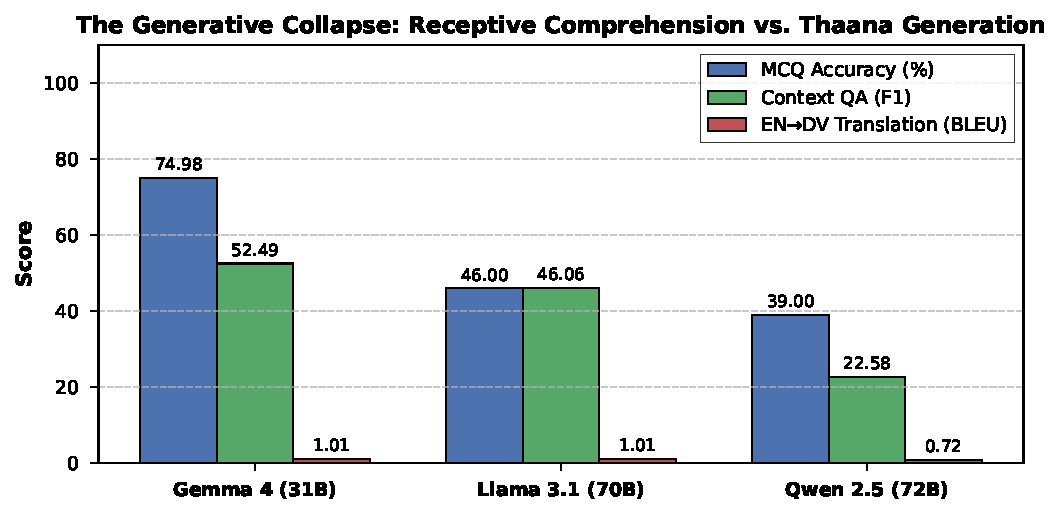
\includegraphics[width=0.85\linewidth]{fig_gap.pdf}
\caption{The Receptive-Generative Disparity: Open-weights models achieve substantial Receptive Comprehension (MCQ/QA) but struggle with generating Thaana (EN$\rightarrow$DV BLEU).}
\label{fig:gap}
\end{figure*}

\subsection{Cross-Domain and Granularity Variance in Translation}
\label{sec:domain_granularity}
Breaking down performance by archival collection and translation register shows how syntactic formality interacts with tokenization. On Contextual QA, Gemma 4 scores highest on structured legal and administrative collections---Shariah \& Law (75.28\% F1, 30.43\% EM) and Political Science (62.30\% F1)---and lowest on Literature \& Poetry (48.94\% F1, 11.51\% EM) and Art \& Culture (46.14\% F1), where figurative syntax and compounded suffixes are more frequent.

\paragraph{EN$\rightarrow$DV Generative Variance and Register Sensitivity.}
On $\text{EN}\rightarrow\text{DV}$ translation, formal constitutional syntax triggered the highest persistent repetition rates (Table \ref{tab:domain}), reaching 5.7\% on legal clauses compared to 3.4\% on Presidency press releases and 3.3\% on general prose and speeches (29.11--29.92 chrF across domains). In all domains, generating Thaana lags reverse translation ($\text{DV}\rightarrow\text{EN}$, 38.01--55.64 chrF) by 8.9 to 25.7 chrF points. Outputs that do not enter persistent loops face a second, sociolinguistic problem. Dhivehi selects distinct verbs, pronouns, and Arabic-derived legal vocabulary according to social and institutional status \cite{gnanadesikan_dhivehi_2017}, and English source sentences rarely mark this (for example, ``stated'' may be rendered as everyday \textit{bunyeve} or honorific \textit{vidhaalhuvieve}). A model translating an isolated sentence therefore has no cue for the expected register. An everyday rendering that keeps the meaning still loses $n$-gram credit against a formal reference. While register divergence contributes to surface metric penalties, our error audit demonstrates that tokenization breakdown and vocabulary scarcity remain the primary generative impediments.

\begin{table*}[t]
\centering
\caption{Translation Variance by Source Domain (Gemma 4 31B)}
\label{tab:domain}
\begin{tabular}{lccc}
\toprule
\textbf{Source Domain} & \textbf{EN$\rightarrow$DV (chrF)} & \textbf{EN$\rightarrow$DV Loop Rate} & \textbf{DV$\rightarrow$EN (chrF)} \\
\midrule
Maldivian Constitution (Legal) & 29.92 & 5.7\% & 55.64 \\
Presidency Press Releases (News) & 29.11 & 3.4\% & 50.29 \\
General Prose / Speech & 29.11 & 3.3\% & 38.01 \\
\bottomrule
\end{tabular}
\end{table*}

\paragraph{Sentence-Level versus Paragraph-Level Granularity.}
Table \ref{tab:granularity} separates the 2,016 translation pairs into single sentences ($n=1,812$) and multi-sentence paragraphs ($n=204$). Target-script breakdown occurs at both lengths: Gemma 4 scores 28.97 chrF and 0.87 BLEU (20.02 char-BLEU) on sentences versus 30.93 chrF and 1.90 BLEU (22.17 char-BLEU) on paragraphs; Llama 3.1 scores 27.73 chrF on sentences and 27.56 chrF on paragraphs; and Qwen 2.5 scores 9.41 chrF on sentences and 9.55 chrF on paragraphs. Because repetition loops typically start within the first 3--5 generated Dhivehi words, single sentences fail at nearly the same rate as multi-sentence paragraphs.

\begin{table*}[t]
\centering
\caption{Translation Performance Stratified by Discourse Granularity (EN$\rightarrow$DV)}
\label{tab:granularity}
\begin{tabular}{llccc}
\toprule
\textbf{Model} & \textbf{Discourse Level} & \textbf{Items ($n$)} & \textbf{chrF} & \textbf{BLEU} \\
\midrule
\multicolumn{5}{l}{\textbf{Gemma Family (Google)}} \\
\quad Gemma 4 (31B) & Sentence-level & 1,812 & 28.97 & 0.87 \\
                    & Paragraph-level & 204 & 30.93 & 1.90 \\
\midrule
\multicolumn{5}{l}{\textbf{Llama Family (Meta)}} \\
\quad Llama 3.1 (70B) & Sentence-level & 1,812 & 27.73 & 0.86 \\
                      & Paragraph-level & 204 & 27.56 & 2.00 \\
\midrule
\multicolumn{5}{l}{\textbf{Qwen Family (Alibaba)}} \\
\quad Qwen 2.5 (72B) & Sentence-level & 1,812 & 9.41 & 0.06 \\
                     & Paragraph-level & 204 & 9.55 & 0.16 \\
\bottomrule
\end{tabular}
\end{table*}

\paragraph{DV$\rightarrow$EN Receptive Variance.}
When translating from Dhivehi into English ($\text{DV}\rightarrow\text{EN}$), domain rankings invert (Table \ref{tab:domain}): Gemma 4 scores highest on the Maldivian Constitution (55.64 chrF) and Presidency Press Releases (50.29 chrF), where formulaic legal clauses and institutional names anchor English generation, and lowest on idiomatic General Literacy prose (38.01 chrF).

\subsection{Directional Asymmetry in Translation (DV$\rightarrow$EN)}
Comparing $\text{EN}\rightarrow\text{DV}$ against $\text{DV}\rightarrow\text{EN}$ across all three open-weights models isolates the script bottleneck (Figure \ref{fig:asymmetry}). On Gemma 4 (31B), translating English into Thaana yields 1.01 BLEU and 29.21 chrF, whereas translating the same pairs from Thaana into English reaches 19.04 BLEU and 50.95 chrF. Llama 3.1 (70B) rises from 27.71 chrF ($\text{EN}\rightarrow\text{DV}$) to 38.40 chrF ($\text{DV}\rightarrow\text{EN}$), and Qwen 2.5 (72B) rises from 9.42 chrF to 40.10 chrF.

\begin{figure*}[t]
\centering
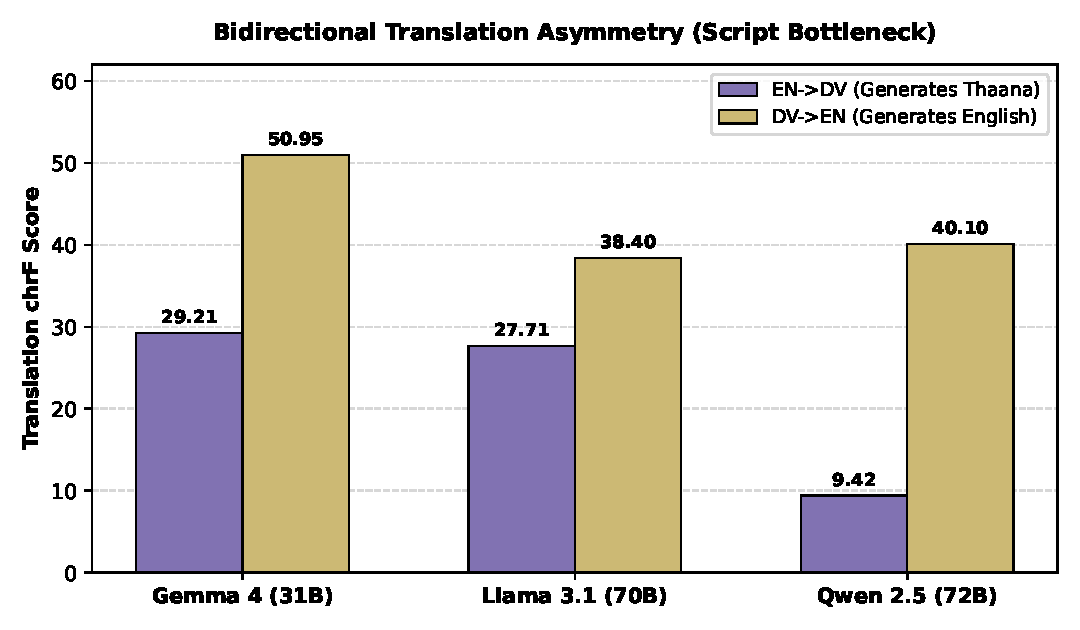
\includegraphics[width=0.85\linewidth]{fig_asymmetry.pdf}
\caption{Directional Translation Asymmetry. Evaluated models translate Dhivehi source text into English (DV$\rightarrow$EN) with substantially higher fidelity than the reverse direction (EN$\rightarrow$DV), consistent with receptive bilingualism.}
\label{fig:asymmetry}
\end{figure*}

ChakmaNMT \cite{chakma_chakmanmt_2026} reports a similar directional gap for the Chakma script: models map fragmented non-Latin input tokens into high-resource English representations during encoding, but lose coherence when required to emit long sequences of unmerged non-Latin tokens during decoding.

\subsection{Qualitative Error Morphology in Thaana Generation}
\label{sec:qualitative_errors}
Two native annotators independently assigned each of 100 failed $\text{EN}\rightarrow\text{DV}$ outputs, sampled across the open-weights cohort, to one of four primary failure categories. They agreed on 72 items (Cohen's $\kappa = 0.63$; chance agreement 24.7\%). Averaged across both annotators, the distribution is:

\begin{enumerate}
    \item \textbf{Repetition Loops (28.0\%; Annotator 1: 32\%, Annotator 2: 24\%):} The model emits 3--5 initial words before repeating a short byte, syllable, or word sequence until hitting the generation limit.
    \item \textbf{Arabic/Latin Script Mixing (28.0\%; Annotator 1: 24\%, Annotator 2: 32\%):} The decoder substitutes Arabic, Indic, or Latin codepoints for Thaana characters (e.g., Arabic \textit{Jeem} \texttt{U+062C} in place of Thaana \textit{Javiyani} \texttt{U+0796}) or splices English words into Thaana clauses.
    \item \textbf{Semantic Drift (23.0\%; Annotator 1: 27\%, Annotator 2: 19\%):} The model produces readable Thaana phrases without loops or foreign scripts, but the meaning diverges from the English source sentence.
    \item \textbf{Morphological Fragmentation (21.0\%; Annotator 1: 17\%, Annotator 2: 25\%):} The model selects recognizable Dhivehi roots in pure Thaana script but attaches mismatched vowel diacritics (\textit{fili}) or broken suffixes, producing non-words.
\end{enumerate}

Disagreements fell mostly along two category boundaries: 17 of the 28 were between Morphological Fragmentation and Semantic Drift, and 5 were between Script Mixing and Repetition Loops. Under a single-label scheme, outputs that show both errors force a choice, which likely explains much of this disagreement. Table \ref{tab:error} shows one such output from Gemma 4 (31B). It begins with an Arabic substitution on the first consonant and then repeats a byte sequence until it reaches 8,192 tokens.

\begin{table*}[t]
\centering
\caption{Taxonomic Failure Example: Gemma 4 (31B) exhibiting Script-Mixing and Repetition Loops. Phonetic romanization and explicit Unicode/UTF-8 codepoints are shown to illustrate script substitution under \texttt{pdflatex}.}
\label{tab:error}
\begin{tabular}{p{0.18\linewidth} p{0.76\linewidth}}
\toprule
\textbf{Source (EN)} & 2. has been convicted of a criminal offence and is serving a sentence of more than twelve months; \\
\midrule
\textbf{Ground Truth (Thaana $\rightarrow$ Romanized)} & 2. [\texttt{U+0796} \textit{Javiyani: \texttt{0xDE 0x96}}] Jinaa'ee kusheh kurikan saabithuve baara masduvahashvure dhigu muddhathehge hukumeh thanfeezukuramundhaa meehaku kamugaivun. \\
\midrule
\textbf{Gemma 4 Output} & 2. [\texttt{U+062C} \textit{Arabic Jeem: \texttt{0xD8 0xAC}}]-naa'ee and varimajuroomukurevifaivaairu, adhi han-recovered han-recovered han-recovered\dots \textit{[Repeats byte sequence to 8,192-token limit]} \\
\bottomrule
\end{tabular}
\end{table*}

\subsection{Ablation: Romanized Transliteration and Multi-Model Script Isolation}
\label{sec:ablation-romanized}
To examine whether target-script generation failure is caused strictly by Thaana sub-syllabic tokenization or compounded by underlying lexical scarcity, we evaluated all three foundation model families---Gemma 4 (31B), Llama 3.1 (70B), and Qwen 2.5 (72B)---on a stratified subset of $n=200$ single-sentence pairs ($<35$ English source words; 50 Constitutional/Legal, 100 Presidency News, 50 Speech/Literature) prompted to generate Dhivehi in the official Mal\'{e} Latin transliteration alphabet (Appendix B). In Table \ref{tab:romanized_ablation}, the Thaana column evaluates the matched 200 items from the main Thaana runs ($\text{max\_tokens} = 8,192$ for Gemma 4; $1,024$ for Llama 3.1 and Qwen 2.5), while the Romanized Mal\'{e} Latin column runs with $\text{max\_tokens} = 256$ under greedy decoding ($\text{temperature} = 0.0$). We scored generations against rule-transliterated Mal\'{e} Latin gold references and computed 95\% confidence intervals via 10,000 paired bootstrap resamples.

Two controls confirm that comparing Thaana ($\ge 1,024$ tokens) against Romanized Latin ($256$ tokens) is not confounded by generation length. First, because Romanized Mal\'{e} Latin averages 1.5--2.0 tokens/word versus 17.8--21.1 tokens/word in Thaana (\S\ref{sec:tokenization_tax}), $\text{max\_tokens} = 256$ in Latin accommodates $\approx$128--170 words ($4\times\text{--}5\times$ the source sentence length), whereas 256 tokens in Thaana would yield only 12--14 Dhivehi words and truncate valid translations mid-clause. Because loop detection counts overlapping sliding 4-grams of whitespace words, repeating a single particle $\ge 50$ times requires only $50 + 3 = 53$ words ($\approx$53--100 Latin tokens), allowing persistent ($\ge 50\times$) loops to fire well within the 256-token Romanized budget (up to 123 repeats on Gemma 4). Second, because greedy decoding ($\text{temperature} = 0.0$) is strictly prefix-invariant, truncating all 200 Thaana outputs to their first 128 whitespace words (matching the word capacity of 256 Latin tokens) yields local ($\ge 5\times$) loop rates of 4.5\% (Gemma 4), 27.0\% (Llama 3.1), and 78.0\% (Qwen 2.5) and persistent ($\ge 50\times$) rates of 4.0\%, 0.0\%, and 10.5\%---within 0.5 percentage points of the uncapped Thaana rates in Table \ref{tab:romanized_ablation}. Because exact word-level BLEU is sensitive to orthographic free variation in romanization schemes (discussed below), character-level chrF serves as our primary ablation metric.

\begin{table*}[t]
\centering
\small
\setlength{\tabcolsep}{2.8pt}
\caption{Romanized Transliteration Ablation Results ($n=200$ stratified single-sentence subset across Legal, News, and Speech) with 95\% Paired Bootstrap Confidence Intervals (10,000 resamples). Evaluating all three open-weights models under the official Mal\'{e} Latin transliteration scheme isolates script-level byte tokenization from underlying linguistic fluency. Loop Rate cells report both local ($\ge 5\times$) and persistent ($\ge 50\times$) sliding 4-gram repetition rates (\texttt{Local / Persistent}).}
\label{tab:romanized_ablation}
\begin{tabular}{l ccc ccc}
\toprule
& \multicolumn{3}{c}{\textbf{Thaana Script ($\ge 1,024$ tok$^\dagger$)}} & \multicolumn{3}{c}{\textbf{Romanized Mal\'{e} Latin ($256$ tok)}} \\
\cmidrule(lr){2-4} \cmidrule(lr){5-7}
\textbf{Model} & \textbf{chrF} & \textbf{BLEU} & \textbf{Loop Rate$^\ddagger$} & \textbf{chrF [95\% CI]} & \textbf{BLEU [95\% CI]} & \textbf{Loop Rate$^\ddagger$} \\
& & & \footnotesize($\ge 5\times$ / $\ge 50\times$) & & & \footnotesize($\ge 5\times$ / $\ge 50\times$) \\
\midrule
Gemma 4 (31B) & 27.97 & 0.56 & 4.5\% / 4.5\% & 15.75 [14.92, 16.62] & 0.15 [0.06, 0.28] & 38.5\% / 18.5\% \\
Llama 3.1 (70B) & 26.65 & 0.75 & 27.0\% / 0.0\% & 17.02 [16.08, 17.98] & 0.26 [0.08, 0.51] & 23.5\% / 5.5\% \\
Qwen 2.5 (72B) & 9.83 & 0.08 & 78.5\% / 11.0\% & \textbf{18.51} [17.78, 19.22] & 0.22 [0.07, 0.44] & 30.0\% / 4.0\% \\
\bottomrule
\end{tabular}
\begin{flushleft}
\footnotesize
$^\dagger$Thaana generations use $\text{max\_tokens} = 8,192$ (Gemma 4) and $1,024$ (Llama 3.1, Qwen 2.5) to offset 14.6x--16.5x token fertility. Under a prefix-invariant 128-word truncation control matching the 256-token Latin word capacity, Thaana loop rates ($\ge 5\times$ / $\ge 50\times$) are 4.5\% / 4.0\% (Gemma 4), 27.0\% / 0.0\% (Llama 3.1), and 78.0\% / 10.5\% (Qwen 2.5).\\
$^\ddagger$For Gemma 4 in Thaana, the local ($\ge 5\times$) and persistent ($\ge 50\times$) rates are both 4.5\% (9/200 items) because 0 items repeat a 4-gram 5--49 times: all 9 looping outputs repeat continuously until hitting the token limit (62--2,036 repeats; across all $N=2,016$ items, $\ge 5\times$ is 3.67\% and $\ge 50\times$ is 3.62\%).
\end{flushleft}
\end{table*}

Switching from Thaana to Latin script produces distinct behavioral shifts across architectures. For Qwen 2.5 (72B), whose tokenizer contains only 8 isolated Thaana consonants and forces byte fallback on 100\% of vowel diacritics, Romanized output improves character-level overlap: chrF nearly doubles from 9.83 to 18.51 (95\% CI: [17.78, 19.22]), while repetition loops drop from 78.5\% down to 30.0\% under $\ge 5\times$ (and from 11.0\% to 4.0\% under $\ge 50\times$), confirming that byte fragmentation in Thaana represented its primary decoding bottleneck. For Llama 3.1 (70B) and Gemma 4 (31B), chrF drops from $\approx$27 to 15.75--17.02; as observed in \S\ref{sec:domain_granularity}, Thaana chrF is buoyed by high-fertility character n-grams matching common vowel diacritics, whereas Romanized chrF reflects non-Thaana text with lower character overlap. For Gemma 4, Thaana generations on this 200-item subset exhibit a 4.5\% loop rate under both $\ge 5\times$ and $\ge 50\times$ thresholds (consistent with the 3.6\% persistent rate across the full 2,016-item track; Table \ref{tab:domain}), as its non-looping failures terminate early after cross-script character substitutions (splicing Arabic, Indic, or Latin codepoints; \S\ref{sec:qualitative_errors}). Under Romanized Latin, Gemma 4 makes zero cross-script byte substitutions, but shifts into morphological particle loops in Latin script (38.5\% under $\ge 5\times$; 18.5\% under $\ge 50\times$), repeatedly emitting grammatical clitics.

\paragraph{Metric Disconnect: Word-BLEU as a Scoring Artifact.}
Word-level BLEU remains suppressed across all three models ($\leq 0.26$). However, this low score is partially an artifact of strict 1-to-1 surface matching against a single rule-transliterated Mal\'{e} Latin reference. The official Mal\'{e} Latin scheme possesses recognized orthographic free variation: models frequently produce phonetically valid spellings that differ in vowel length notation (\textit{ee} vs. \textit{ey}, \textit{oo} vs. \textit{oa}), consonant gemination, apostrophes for \textit{Sukun}, or compound hyphenation. Under standard 13a tokenized word BLEU, any minor orthographic variance scores exactly zero. In contrast, character-level chrF (15.75--18.51) is spelling-tolerant and rewards partial morphemic overlap, making it the more reliable indicator of generational quality.

\begin{table*}[t]
\centering
\small
\caption{Representative Romanized Dhivehi Model Generations ($n=200$ Ablation) Illustrating Orthographic Free Variation, English Code-Switching with Dhivehi Suffixation, and Grammatical Particle Loops.}
\label{tab:romanized_examples}
\begin{tabular}{p{0.22\linewidth} p{0.73\linewidth}}
\toprule
\textbf{Category} & \textbf{Source, Gold Reference, and Model Generations} \\
\midrule
\textbf{Synonymy \& Register Divergence} & \textbf{Source (EN):} 2. the purpose and importance of limiting the right or freedom; \\
& \textbf{Gold (Mal\'{e} Latin):} 2. e \underline{haggheh} nuvatha e minivankameh hifehettumuge \underline{beynumaa'i}, \underline{muhinmukan}. \\
& \textbf{Gemma 4 (31B):} 2. \underline{hakku} eh nungaa adha libarun limiting kurun ge \underline{maqsadu} adha ege \underline{ahmiyyath}; \\
& \textit{\footnotesize Qualitative note: Model retrieves valid Arabic loan synonyms (\textit{hakku} [right], \textit{maqsadu} [purpose], \textit{ahmiyyath} [importance]) where the formal legal reference uses native Dhivehi phrasing (\textit{haggheh}, \textit{beynumaa'i}, \textit{muhinmukan}), yielding 0.0 word-BLEU despite semantic alignment.} \\
\midrule
\textbf{English Code-Switching \& Dhivehi Inflection} & \textbf{Source (EN):} The jurisdiction of the Judicial Service Commission shall extend to all members of the Judiciary and such other persons as designated by the People’s Majlis. \\
& \textbf{Gold (Mal\'{e} Latin):} ghadhulu indaafu ghaa'imkurumuge baaruga'i himeney enmeha'i meehunaa'i, rayyithunge majileehun kanda'alhaa konme faraathegge macchash judeesal sarvis komisanuge ikhthidaad hingaane'eve. \\
& \textbf{Gemma 4 (31B):} \underline{Judicial Service Commission-ge} \underline{jurisdiction-aa} hifaa-fai vanee, Judiciary-ge gaana-gaana \underline{members-ah} aa People's Majlis-a\dots \\
& \textit{\footnotesize Qualitative note: Model retains English technical nouns but attaches productive Dhivehi case clitics (genitive \textit{-ge}, conjunctive \textit{-aa}, dative \textit{-ah}), reflecting syntactic grammatical frame competence alongside lexical retrieval failure.} \\
\midrule
\textbf{Morphological Particle Loops} & \textbf{Source (EN):} (h) to issue declarations of war and peace, and to immediately submit such declarations to the People’s Majlis for approval; \\
& \textbf{Gold (Mal\'{e} Latin):} (') hanguraama nuvatha dulha ighulaankurumuge gharaaru nerumaa'i, efadha gharaaruthah rayyithunge majileehun faaskurumahtaka'i e majileehash evaguthun hushahelhun. \\
& \textbf{Gemma 4 (31B):} (h) war eh \underline{thah thah thah thah thah thah thah thah thah thah thah thah}\dots \\
& \textit{\footnotesize Qualitative note: In Latin script, decoders avoid byte-level Unicode loops but remain vulnerable to grammatical particle loops, repeatedly generating the plural marker \textit{thah}.} \\
\bottomrule
\end{tabular}
\end{table*}

\paragraph{Qualitative Audit of Romanized Outputs.}
To characterize residual errors beyond scoring artifacts, two native speakers (Annotator 1 and Annotator 2) independently audited a stratified sample of 50 Romanized generations across all three models. Annotators achieved an observed agreement of 66.0\% (Cohen's $\kappa = 0.50$; chance agreement 32.0\%, reaching 80.0\% agreement on Gemma 4; full confusion matrix in Appendix C). Averaged across both annotators (100 total ratings), the mutually exclusive categorization reveals:
\begin{enumerate}
    \item \textbf{Morphological Particle Loops (40.0\%; Annotator 1: 44.0\%, Annotator 2: 36.0\%):} Although Latin output eliminates byte-level Unicode loops, decoders remain vulnerable to grammatical particle loops in Latin text, repeatedly emitting plural markers (\textit{thah thah thah}), verbal copulas (\textit{kuraa kuraa}), or reduplicated clitics (\textit{fali-fali}). This failure mode dominates Gemma 4, accounting for 55.0\% of its evaluated generations.
    \item \textbf{Semantic Incoherence and Hallucination (37.0\%; Annotator 1: 36.0\%, Annotator 2: 38.0\%):} The model generates phonetically plausible Latin strings that do not correspond to any valid Dhivehi root or English transfer, producing severe morphological distortions (46.9\% on Llama 3.1 and 50.0\% on Qwen 2.5).
    \item \textbf{English Code-Switching and Hybrid Inflection (15.0\%; Annotator 1: 16.0\%, Annotator 2: 14.0\%):} Rather than retrieving native Dhivehi vocabulary, models retain English noun stems and attach valid Dhivehi grammatical suffixes (e.g., generating \textit{disability thah} instead of \textit{nukulhedhuntherikan}, \textit{flats-ah} instead of \textit{imaaraathah}, or \textit{Judicial Service Commission-ge} and \textit{members-ah}; Table \ref{tab:romanized_examples}). On Gemma 4, this code-switching characterizes 22.5\% of generations, demonstrating correct receptive assignment of case and plurality roles despite lexical retrieval failure.
    \item \textbf{Synonymy and Register Divergence (7.0\%; Annotator 1: 2.0\%, Annotator 2: 12.0\%):} Models produce valid everyday Dhivehi roots or established Arabic loanwords that diverge lexically from formal constitutional gold references (e.g., generating \textit{hakku} [right], \textit{maqsadu} [purpose], and \textit{ahmiyyath} [importance] where the official legal reference uses formal phrasing \textit{haggheh}, \textit{beynumaa'i}, and \textit{muhinmukan}; Table \ref{tab:romanized_examples}).
    \item \textbf{Fluent and Accurate Translation (1.0\%; Annotator 1: 2.0\%, Annotator 2: 0.0\%):} Only a single generation achieved full semantic fidelity and natural Mal\'{e} Latin syntax, confirming that low word-BLEU ($\le 0.26$) is not merely a surface scoring artifact, but reflects substantive generative breakdown in Latin text.
\end{enumerate}

These findings qualify the script-isolation hypothesis: while byte-fallback tokenization triggers the severe decoding breakdown and infinite loops observed in Thaana script, foundation models also suffer from deep lexical scarcity and register limitations in Dhivehi. Generative fluency cannot be restored merely by altering the surface orthography without substantial pre-training vocabulary expansion.

\section{Limitations}
\label{sec:limitations}

\paragraph{Multimodal Pre-Training and Zero-Shot OCR Bounds.}
Several current open-weights models, including Gemma 4, incorporate vision encoders trained on document images. If unindexed PDF scans from \textit{Saruna} appeared in multimodal pre-training corpora, visual contamination could occur in principle. In practice, general-purpose vision-language models lack Thaana OCR alignment and fail on historical Dhivehi scans \cite{hameed_bridging_2026}, dropping stacked diacritics and misreading \textit{Hus Noonu}---the exact failure that required us to use the fine-tuned Viyavi OCR pipeline (8.0\% initial CER, reduced to 1.4\% CER after human post-editing).

\paragraph{Register Skew and Dialectal Coverage.}
Sourcing comprehension passages from university archives, legal statutes, and academic monographs biases Dhivehi-Bench toward formal Mal\'{e} Dhivehi. The benchmark does not test informal chat registers, Latin-Thaana code-switching, or the southern dialects of Huvadhoo, Fuvahmulah, and Addu, which differ substantially in phonology and inflectional morphology \cite{fritz_dhivehi_2002}.

\paragraph{Single-Reference Span Granularity and Diglossic Register Sensitivity.}
Each Contextual QA and Translation item in Dhivehi-Bench is scored against a single gold reference. On Contextual QA, as shown by our human baseline audit (\S\ref{sec:human_baseline}), single-reference whitespace F1 penalizes valid boundary-length choices (extracting a minimal entity vs. a full framing clause), optional copula suffixes (\textit{-eve}), and compound word spacing, capping strict Token F1 near 52.6\% even though 88.0\% of the human responses overlap lexically with the reference span. Similarly, on the Translation track, isolated English source sentences do not specify which tier of Dhivehi's diglossic honorific register (\textit{Reethi Bas} vs. everyday speech) is expected, so surface $n$-gram metrics penalize valid everyday translations when the single reference uses formal or honorific vocabulary. Future iterations of Dhivehi-Bench will add multi-reference QA annotations (pairing minimal entity and clause-level spans) and register-tagged translation references.

\paragraph{Public-Domain Status of the Translation Track.}
Unlike the offline archival MCQ and QA tracks, the Translation track draws from the Maldivian Constitution, Presidency press releases, and published translations that exist on the public web. Any pre-training exposure to these parallel texts did not aid Thaana generation: all three models scored $\leq 1.01$ BLEU on $\text{EN}\rightarrow\text{DV}$ translation, succumbing to severe autoregressive degradation and script substitutions on Gemma 4 and Qwen 2.5. Future benchmark releases will add newly commissioned, unpublished human translations.

\paragraph{Inferential Nature of the Attention Dilation Hypothesis.}
While our Romanized transliteration ablation (\S\ref{sec:ablation-romanized}) demonstrates that eliminating Thaana script output removes cross-script byte substitutions and cuts repetition loops on byte-fallback-bound Qwen 2.5 (78.5\% to 30.0\% local; 11.0\% to 4.0\% persistent), our multi-model evaluation shows that models still encounter grammatical particle loops (Gemma 4 at 38.5\% local; 18.5\% persistent), lexical hallucination, and code-switching in Latin script. Testing the self-attention dilation mechanism directly requires white-box analyses---tracking attention entropy and logit-lens projections across layers, or training controlled vocabulary-expansion and byte-latent models (ByT5 \cite{xue_byt5_2022}, Byte Latent Transformer \cite{pagnoni_byte_2025}) on matched corpora.

\section{Conclusion and Future Work}
We introduced Dhivehi-Bench, a 5,220-item multi-task benchmark for evaluating Large Language Models on the Maldivian language across multiple-choice reading comprehension ($n=2,070$), contextual question answering ($n=1,134$), and bidirectional translation ($n=2,016$). Digitizing offline physical archives via custom Thaana OCR and validating every item across three native speakers to 100\% consensus provides a contamination-mitigated testbed for a script with zero multi-character merges in current open-weights tokenizers. Our baseline evaluations across Gemma 4 (31B), Llama 3.1 (70B), and Qwen 2.5 (72B) show a consistent asymmetry between receptive comprehension and target-script generation: Gemma 4 achieves 74.98\% MCQ accuracy, 52.49\% QA Token F1, and 50.95 chrF on $\text{DV}\rightarrow\text{EN}$ translation, yet collapses to 1.01 BLEU when generating Thaana ($\text{EN}\rightarrow\text{DV}$), succumbing to repetitive loops and foreign script substitutions. Evaluating an orthographic ablation via Romanized Mal\'{e} Latin transliteration across all three models ($n=200$, 10,000 paired bootstrap resamples) shows that Latin output eliminates cross-script byte substitutions and reduces repetition loops for byte-fallback-bound Qwen 2.5 (from 78.5\% to 30.0\% local; 11.0\% to 4.0\% persistent), while shifting Gemma 4 into Latin grammatical particle loops (38.5\% local; 18.5\% persistent) and leaving word-level BLEU $\leq 0.26$. Our double-blind human error audit ($n=50$, Cohen's $\kappa=0.50$) confirms that Romanized generations remain dominated by morphological particle loops (40.0\%), lexical hallucination (37.0\%), and English code-switching (15.0\%), demonstrating that generative failure reflects both script-level tokenization and pre-training data scarcity.

Dhivehi-Bench provides an empirical baseline for testing tokenizer and architectural interventions on non-Latin scripts, including byte-to-patch models (H-Net \cite{hwang_dynamic_2025}, Byte Latent Transformer \cite{pagnoni_byte_2025}), morpheme-aware vocabularies (MorphBPE \cite{asgari_morphbpe_2026}, MoVoC \cite{teklehaymanot_movoc_2025}), and byte-level pretokenization reforms (SCRIPT-BPE \cite{land_bpe_2025}, MYTE \cite{limisiewicz_myte_2024}), alongside dynamic contamination-free evaluation updates \cite{li_latesteval_2023, chen_benchmarking_2025}.

\section{Data and Code Availability}
We release the Dhivehi-Bench dataset (2,070 MCQ items, 1,134 Contextual QA pairs, and 2,016 parallel translation pairs) on Hugging Face Datasets under a CC-BY-NC 4.0 license upon publication (anonymized review URL: \url{https://anonymous.4open.science/r/dhivehi-bench-data}). The evaluation harness, prompt templates, and tokenizer verification script (\texttt{scripts/verify\_tokenizers.py}) are available at \url{https://anonymous.4open.science/r/dhivehi-bench} under the MIT License.

To comply with copyright law, we distribute only transformed derivative QA pairs and short context excerpts under Fair Use for non-consumptive computational research; official governmental communications and constitutional texts are in the public domain.

\begin{acks}
Funding sources, institutional affiliations, and individual annotator acknowledgments are omitted for double-blind review and will be restored in the camera-ready version upon publication.
\end{acks}

\bibliographystyle{ACM-Reference-Format}
\bibliography{references}

\section*{Appendix A: Prompt Templates}

\noindent\textbf{Translation (DV$\rightarrow$EN):}\\
\texttt{Translate the following Dhivehi text into English.}\\
\texttt{Dhivehi: [target\_text]}\\
\texttt{English:}

\vspace{6pt}
\noindent\textbf{Translation (EN$\rightarrow$DV):}\\
\texttt{Translate the following English text into Dhivehi.}\\
\texttt{English: [source\_text]}\\
\texttt{Dhivehi:}

\vspace{6pt}
\noindent\textbf{Contextual QA:}\\
\texttt{Read the following Dhivehi paragraph and answer the question in Dhivehi.}\\
\texttt{Context: [context]}\\
\texttt{Question: [question]}\\
\texttt{Answer:}

\vspace{6pt}
\noindent\textbf{Multiple Choice (MCQ):}\\
\texttt{Question: [question]}\\
\texttt{A. [option\_a]}\\
\texttt{B. [option\_b]}\\
\texttt{C. [option\_c]}\\
\texttt{D. [option\_d]}\\
\texttt{Answer:}


\vspace{6pt}
\noindent\textbf{Translation --- Romanized Mal\'{e} Latin Ablation (\S\ref{sec:ablation-romanized}):}\\
\texttt{Translate the following English text into Dhivehi using the standard Mal\'{e} Latin transliteration alphabet (Romanized Dhivehi). Output only the Romanized Dhivehi translation without Thaana script.}\\
\texttt{English: [source\_text]}\\
\texttt{Romanized Dhivehi:}

\section*{Appendix B: Mal\'{e} Latin Transliteration Mapping}
The Romanized transliteration ablation (\S\ref{sec:ablation-romanized}) adopted the standardized Mal\'{e} Latin orthographic mapping used in official administrative and educational contexts in the Maldives \cite{gnanadesikan_dhivehi_2017}. Table \ref{tab:transliteration} documents the phonetic correspondence for all 24 primary consonants and 11 vowel diacritics, followed by the orthographic rules for \textit{Sukun}, \textit{Hus Noonu}, and Arabic-derived dotted consonants (\textit{Tikhi Thaana}).

\begin{table*}[h]
\centering
\small
\caption{Official Mal\'{e} Latin Transliteration Scheme for Dhivehi (Thaana Script).}
\label{tab:transliteration}
\begin{tabular}{llcllc}
\toprule
\textbf{Thaana Consonant} & \textbf{Name} & \textbf{Latin} & \textbf{Thaana Diacritic} & \textbf{Name} & \textbf{Latin} \\
\midrule
Haa (\texttt{U+0780}) & Haa & h & Aba-fili (\texttt{U+07A6}) & Aba-fili & a \\
Shaviyani (\texttt{U+0781}) & Shaviyani & sh & Aabaa-fili (\texttt{U+07A7}) & Aabaa-fili & aa \\
Noonu (\texttt{U+0782}) & Noonu & n & Ibi-fili (\texttt{U+07A8}) & Ibi-fili & i \\
Raa (\texttt{U+0783}) & Raa & r & Eebee-fili (\texttt{U+07A9}) & Eebee-fili & ee \\
Baa (\texttt{U+0784}) & Baa & b & Ubu-fili (\texttt{U+07AA}) & Ubu-fili & u \\
Lhaviyani (\texttt{U+0785}) & Lhaviyani & lh & Ooboo-fili (\texttt{U+07AB}) & Ooboo-fili & oo \\
Kaafu (\texttt{U+0786}) & Kaafu & k & Ebe-fili (\texttt{U+07AC}) & Ebe-fili & e \\
Alifu (\texttt{U+0787}) & Alifu & ' & Eybey-fili (\texttt{U+07AD}) & Eybey-fili & ey \\
Vaavu (\texttt{U+0788}) & Vaavu & v & Obo-fili (\texttt{U+07AE}) & Obo-fili & o \\
Meemu (\texttt{U+0789}) & Meemu & m & Oaboa-fili (\texttt{U+07AF}) & Oaboa-fili & oa \\
Faafu (\texttt{U+078A}) & Faafu & f & Sukun (\texttt{U+07B0}) & Sukun & \textit{(stop/geminate)} \\
Dhaalu (\texttt{U+078B}) & Dhaalu & dh & & & \\
Thaa (\texttt{U+078C}) & Thaa & th & & & \\
Laamu (\texttt{U+078D}) & Laamu & l & & & \\
Gaafu (\texttt{U+078E}) & Gaafu & g & & & \\
Gnaviyani (\texttt{U+078F}) & Gnaviyani & gn & & & \\
Seenu (\texttt{U+0790}) & Seenu & s & & & \\
Daviyani (\texttt{U+0791}) & Daviyani & d & & & \\
Zaaviyani (\texttt{U+0792}) & Zaaviyani & z & & & \\
Ttaviyani (\texttt{U+0793}) & Ttaviyani & t & & & \\
Yaavu (\texttt{U+0794}) & Yaavu & y & & & \\
Paviyani (\texttt{U+0795}) & Paviyani & p & & & \\
Javiyani (\texttt{U+0796}) & Javiyani & j & & & \\
Chaviyani (\texttt{U+0797}) & Chaviyani & ch & & & \\
\bottomrule
\end{tabular}
\end{table*}

\vspace{4pt}
\noindent\textbf{Orthographic Rules for Sukun (\texttt{U+07B0}), Hus Noonu (\texttt{U+0782}), and Dotted Consonants (\textit{Tikhi Thaana}):}
\begin{itemize}
    \item \textbf{Sukun (\texttt{U+07B0}) Realization:} Word-medially before a consonant, \textit{sukun} triggers gemination of the following consonant (e.g., \textit{rah} + \textit{thah} $\rightarrow$ \textit{rahthah}). Word-finally, \textit{Alifu sukun} (\texttt{U+0787 U+07B0}) and \textit{Shaviyani sukun} (\texttt{U+0781 U+07B0}) transliterate to word-final \texttt{-h} (glottal stop), \textit{Noonu sukun} (\texttt{U+0782 U+07B0}) to \texttt{-n}, \textit{Thaa sukun} (\texttt{U+078C U+07B0}) to \texttt{-iy} / \texttt{-th}, and \textit{Seenu sukun} (\texttt{U+0790 U+07B0}) to \texttt{-s}.
    \item \textbf{Hus Noonu (\texttt{U+0782} without fili/sukun):} Transliterated as prenasalized \texttt{n} preceding voiced stops (\texttt{nd}, \texttt{ndh}, \texttt{mb}, \texttt{ng}, as in \textit{kandu} and \textit{handhu}).
    \item \textbf{Arabic-Derived Dotted Thaana (\textit{Tikhi Thaana}, \texttt{U+0798}--\texttt{U+07A5} and \texttt{U+07B1}):} Mapped to their standard phonetic Latin counterparts in legal and Islamic texts: \textit{Thaalu} (\texttt{U+0798} $\rightarrow$ \texttt{th}/\texttt{dh}), \textit{Hhaa} (\texttt{U+0799} $\rightarrow$ \texttt{h}), \textit{Khaa} (\texttt{U+079A} $\rightarrow$ \texttt{kh}), \textit{Dhaal} (\texttt{U+079B} $\rightarrow$ \texttt{dh}/\texttt{z}), \textit{Sheenu} (\texttt{U+079C} $\rightarrow$ \texttt{sh}), \textit{Saadhu} (\texttt{U+079D} $\rightarrow$ \texttt{s}), \textit{Daadhu} (\texttt{U+079E} $\rightarrow$ \texttt{d}), \textit{To} (\texttt{U+079F} $\rightarrow$ \texttt{t}), \textit{Zo} (\texttt{U+07A0} $\rightarrow$ \texttt{z}), \textit{Ainu} (\texttt{U+07A1} $\rightarrow$ \texttt{'}), \textit{Ghainu} (\texttt{U+07A2} $\rightarrow$ \texttt{gh}), \textit{Qaafu} (\texttt{U+07A3} $\rightarrow$ \texttt{q}), \textit{Ghaafu} (\texttt{U+07A4} $\rightarrow$ \texttt{gh}), \textit{Waavu} (\texttt{U+07A5} $\rightarrow$ \texttt{w}), and \textit{Naa} (\texttt{U+07B1} $\rightarrow$ \texttt{n}).
\end{itemize}

\section*{Appendix C: Inter-Annotator Agreement on Romanized Transliteration Audit}
Table \ref{tab:confusion_matrix} documents the empirical confusion matrix between the two independent native evaluators (Annotator 1 and Annotator 2) across the 50 Romanized translation outputs (\S\ref{sec:ablation-romanized}).

\begin{table}[h]
\centering
\small
\setlength{\tabcolsep}{5pt}
\caption{Inter-Annotator Confusion Matrix for Romanized Error Morphology Audit ($n=50$, Cohen's $\kappa=0.50$, Observed Agreement 66.0\%). Rows represent Annotator 1 and columns represent Annotator 2.}
\label{tab:confusion_matrix}
\begin{tabular}{lccccc}
\toprule
\textbf{Annotator 1 $\backslash$ Annotator 2} & \textbf{Loops} & \textbf{Code-Switch} & \textbf{Incoherent} & \textbf{Synonymy} & \textbf{Fluent} \\
\midrule
Morphological Loops & 17 & 1 & 4 & 0 & 0 \\
Code-Switching & 0 & 4 & 2 & 2 & 0 \\
Incoherent / Hallucination & 1 & 1 & 12 & 4 & 0 \\
Synonymy / Register & 0 & 1 & 0 & 0 & 0 \\
Fluent Translation & 0 & 0 & 1 & 0 & 0 \\
\bottomrule
\end{tabular}
\end{table}

\end{document}
